  \section{Eindimensionale Richtungsbestimmung} \todo{Robin: Bleibt, Ortung -> Richtung}
  Um den Algorithmus, der aus den Phasendifferenzen den Ort zurückrechnet zu entwickeln haben wir mit der
einfachsten Stufe der Ortung, die eindimensionale Ortung, angefangen:
    \begin{figure}
        \centering
        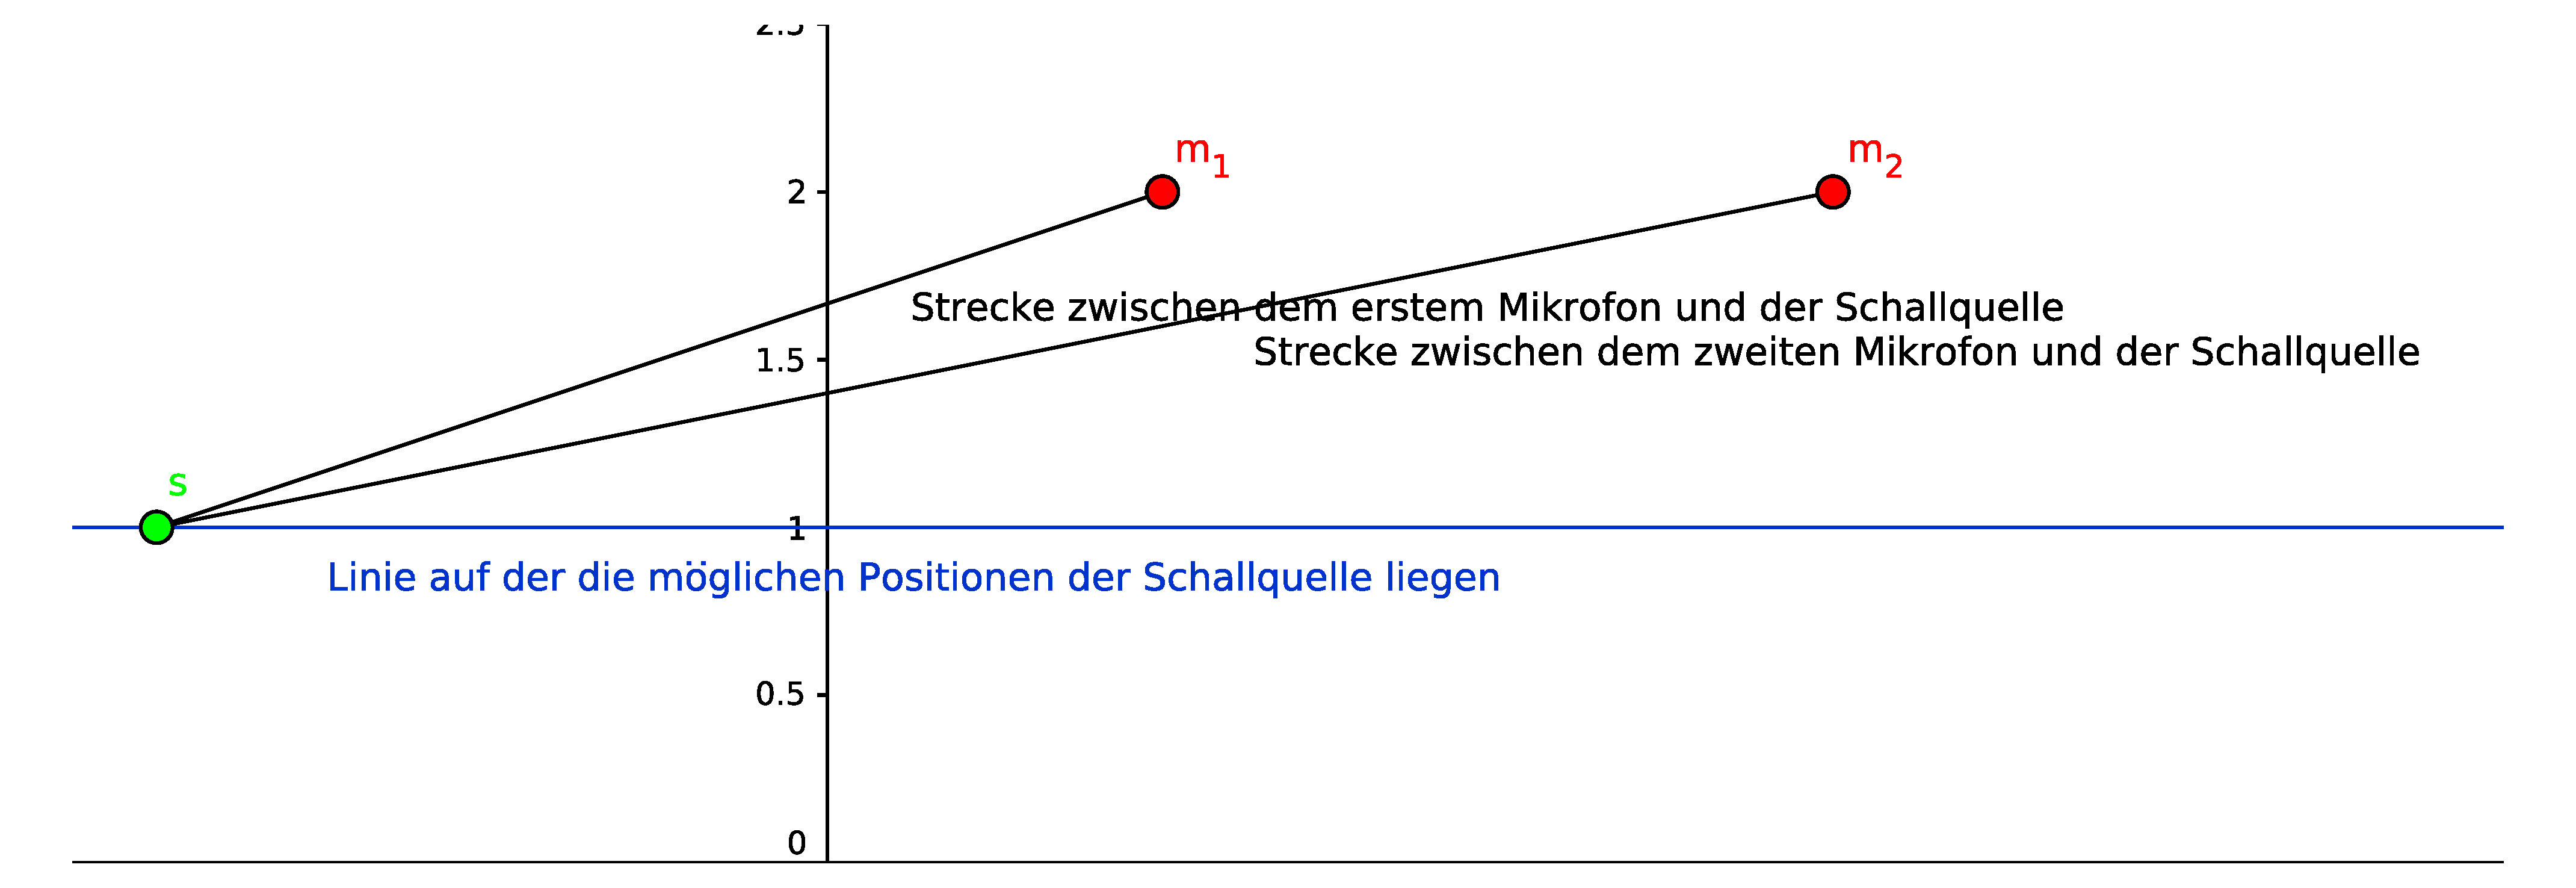
\includegraphics[width=\linewidth]{skizze1d}
        \caption{Skizze einer eindimensionalen Ortung}
    \end{figure}
